\documentclass[11pt]{article}
\usepackage[margin=1in]{geometry}
\usepackage{mathpazo}
\usepackage{amsmath,amssymb}
\usepackage{microtype}
\usepackage{booktabs}
\usepackage{graphicx}
\usepackage[dvipsnames]{xcolor}
\usepackage{tikz}
\usetikzlibrary{positioning,arrows.meta,calc,fit,backgrounds}
\usepackage[most]{tcolorbox}
\usepackage{enumitem}
\usepackage{listings}
\usepackage[font=small,labelfont=bf]{caption}
\usepackage{hyperref}
\hypersetup{colorlinks=true,linkcolor=MidnightBlue,citecolor=MidnightBlue,urlcolor=MidnightBlue}
\usepackage{cleveref}
\urlstyle{tt}
\def\UrlBreaks{\do\_\do/\do.}
\newcommand{\file}[1]{\nolinkurl{#1}}
\newcommand{\code}[1]{\texttt{#1}}
\newcommand{\mhh}{m_{hh}}
\newcommand{\bw}{\boldsymbol{\omega}}
\newcommand{\bp}{\boldsymbol{p}}
\newcommand{\bx}{\boldsymbol{x}}
\newcommand{\data}{\mathcal{D}}

\definecolor{trainable}{HTML}{1B6CA8}
\definecolor{physics}{HTML}{2E933C}
\definecolor{datac}{HTML}{7B4EA3}
\definecolor{warn}{HTML}{C0392B}

\newtcolorbox{keyidea}[1][]{enhanced,breakable,colback=physics!6,colframe=physics!70!black,
  fonttitle=\bfseries,title={#1},boxrule=0.6pt,arc=2pt,left=6pt,right=6pt}
\newtcolorbox{aside}[1][]{enhanced,breakable,colback=trainable!5,colframe=trainable!70!black,
  fonttitle=\bfseries,title={#1},boxrule=0.6pt,arc=2pt,left=6pt,right=6pt}
\newtcolorbox{assume}[1][]{enhanced,breakable,colback=datac!5,colframe=datac!70!black,
  fonttitle=\bfseries,title={#1},boxrule=0.6pt,arc=2pt,left=6pt,right=6pt}
\newtcolorbox{watch}[1][]{enhanced,breakable,colback=warn!5,colframe=warn!70!black,
  fonttitle=\bfseries,title={#1},boxrule=0.6pt,arc=2pt,left=6pt,right=6pt}
\setlist{itemsep=2pt,topsep=3pt}
\setlength{\emergencystretch}{3em}

\lstset{language=Python, basicstyle=\ttfamily\small, columns=fullflexible,
  keepspaces=true, commentstyle=\color{physics!70!black}\itshape,
  keywordstyle=\color{trainable!90!black}\bfseries, stringstyle=\color{datac},
  showstringspaces=false, frame=single, rulecolor=\color{gray!40},
  backgroundcolor=\color{gray!3}, xleftmargin=4pt, xrightmargin=4pt,
  aboveskip=6pt, belowskip=6pt}

\title{\textbf{The smooth $23\times80$ model: first results}\\[4pt]
\large Accuracy, calibration, within-bin and edge tests, sensitivity}
\author{P.~Bhat, N.~De~Filippis, K.\,F.~Johnson, H.\,B.~Prosper, R.~Starnes}
\date{October 31, 2026}
\begin{document}
\maketitle

\begin{keyidea}[In brief]
\begin{enumerate}
  \item \textbf{It works, and it is the best model we have.} On the 1,000 test spectra the
    smooth model ($J = 40$ splines per function, threshold factor) is as accurate as the best
    alternative (Poisson deviance per bin 1.566 below and 1.100 above 555~GeV, against 1.559
    and 1.105 for the free per-bin fit with Poisson weights), with an exact fit uncertainty of
    2.9\% of the noise. With the discrepancy its pulls have s.d.\ 1.004 (1.011 below, 1.001
    above 555~GeV), 95.4\% within $\pm2$, and are calibrated at every degree of cancellation
    ($\langle z^2\rangle$ = 0.97--1.04).
  \item \textbf{It describes the inside of a bin.} Fitted on 30-GeV bins, it predicts how
    each splits into two 15-GeV bins to within the noise above about 360~GeV, where the free
    fit cannot (split $\chi^2$ up to 30). Below 345~GeV the threshold structure is finer than
    30~GeV and the split is predicted less well.
  \item \textbf{The threshold factor matters}; extrapolation above 1455~GeV does not work.
  \item \textbf{A finding on the way: weighting by the observed counts biases fits low.}
    All earlier fits (the network fine-tune, the free fit) used weights $1/(q(t+q))$; with
    tens of events per bin at high mass this biases them low by a measurable amount. The
    smooth model uses the model's own Poisson variances (iterated), and passes a toy test
    with known answers (pull s.d.\ 0.97, mean $+0.06$).
\end{enumerate}
\end{keyidea}

\tableofcontents

% ===========================================================================
\section{Implementation and the toy test}

The model is in \file{dihiggs/smooth.py} (\code{SplineBasis}, \code{SmoothHEFT}); the plan
is \file{docs/smooth/smooth_plan.pdf}. Fitting the 3,989 training spectra (281,044 rows
including 1,814 restored empty bins) takes about a minute on a laptop CPU.

\paragraph{Toy test} (\file{code/smooth_toy.py}). Three known smooth coefficient functions,
600 spectra of 40,000 equal-weight events in 15-GeV bins. (i) For fixed smoothness the fit
agrees with a direct dense solve to $6\times10^{-14}$. (ii) With the smoothness chosen by the
evidence, the fitted functions agree with the truth within their quoted uncertainties: pulls
over 80 points $\times$ 3 functions have mean $+0.06$ and s.d.\ 0.97.

\begin{watch}[Weighting by the observed counts biases a fit low]
In the first version of the toy test the pulls had mean $-0.93$, worst at high mass. The
cause is classic: weighting each bin by $1/(q\,n)$, with $n$ the observed count (Neyman's
$\chi^2$), gives downward fluctuations larger weights, so the fit is pulled low by about one
event per bin; with $\sim$20--50 events per bin at high mass and 3,989 spectra pooled, that
is many standard deviations of the fit. The cure is to weight by the model's own Poisson
variance, $q\max(f, q)$, and iterate (\code{fit\_poisson}); at convergence this is the Poisson
maximum-likelihood fit. Where the model predicts a negative value the observed count is used,
and each iteration moves half-way, which avoids oscillation. The network fine-tune and the
free fit used the biased weights; \cref{tab:acc} shows the effect.
\end{watch}

% ===========================================================================
\section{Accuracy}

Because the Neyman $\chi^2$ favours predictions that are biased low, we compare models with
the Poisson deviance, the natural measure for counts, and also show Neyman and Pearson.

\begin{table}[h]
\centering
\small
\begin{tabular}{lccccccc}
\toprule
 & \multicolumn{2}{c}{Neyman} & \multicolumn{2}{c}{Pearson} & \multicolumn{2}{c}{deviance} & median \\
model (weights) & 255--555 & $>555$ & 255--555 & $>555$ & 255--555 & $>555$ & dev./$N$ \\
\midrule
network ensemble (observed counts)  & 1.648 & 1.115 & 1.554 & 1.147 & 1.561 & 1.121 & 1.085 \\
free fit (observed counts)          & 1.581 & 1.121 & 1.562 & 1.223 & 1.542 & 1.150 & 1.096 \\
free fit (Poisson, iterated)        & 1.643 & 1.148 & 1.535 & 1.103 & 1.559 & 1.105 & 1.075 \\
\textbf{smooth, $J = 40$ (Poisson)} & 1.650 & 1.144 & 1.542 & 1.096 & 1.566 & 1.100 & 1.078 \\
smooth, $J = 30$                    & 1.658 & 1.145 & 1.549 & 1.096 & 1.573 & 1.101 & 1.079 \\
smooth, $J = 60$                    & 1.643 & 1.145 & 1.535 & 1.096 & 1.559 & 1.100 & 1.074 \\
smooth, $J = 40$, no threshold factor & 1.648 & 1.144 & 1.541 & 1.096 & 1.564 & 1.100 & 1.078 \\
\bottomrule
\end{tabular}
\caption{Mean per bin on the 1,000 test spectra, below and above 555~GeV, for three measures
of agreement with Poisson counts. The weights used in fitting are given in brackets.}
\label{tab:acc}
\end{table}

\begin{itemize}
  \item The smooth model is as accurate as the free fit with Poisson weights, and better than
    the network above 555~GeV (deviance 1.100 vs 1.121, Pearson 1.096 vs 1.147), where the
    network's biased weights cost it.
  \item With the observed-count weights the free fit looks better in Neyman's measure (1.581)
    and worse in Pearson's (1.223 above 555~GeV): the signature of a downward bias.
  \item The results hardly depend on $J$ (30, 40, 60) and, within 255--1455~GeV, on the
    threshold factor.
\end{itemize}

% ===========================================================================
\section{Calibration}

\begin{figure}[h]
\centering
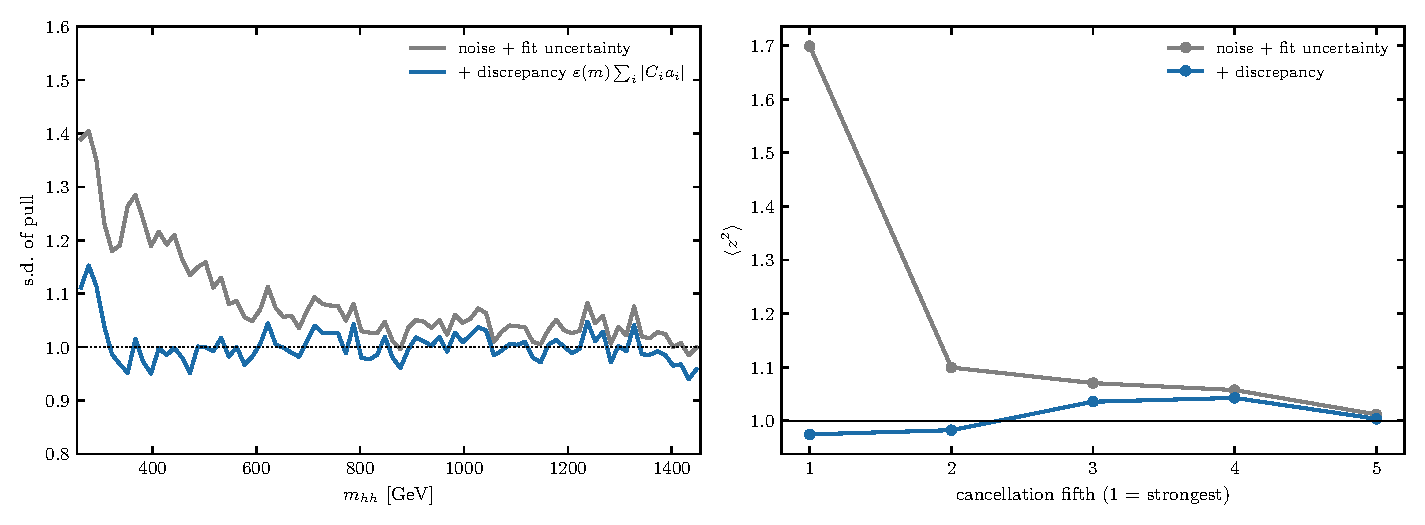
\includegraphics[width=\textwidth]{fig_smooth_calibration.pdf}
\caption{Standard deviation of the pull on the test spectra as a function of $m_{hh}$ (left)
and $\langle z^2\rangle$ by degree of cancellation (right), without and with the discrepancy.}
\label{fig:cal}
\end{figure}

With $z = (t - f)/\sqrt{q f + s^2 + s_\text{disc}^2}$, where $s^2$ is the exact fit variance and
$s_\text{disc} = \varepsilon(m_{hh})\sum_i|C_ia_i|$ fitted on the 38,076 quick-test rows:
s.d.\ 1.004 (1.011 below and 1.001 above 555~GeV), 95.4\% within $\pm2$ (95.4\% expected),
and $\langle z^2\rangle$ = 0.97, 0.98, 1.04, 1.04, 1.00 from the most to the least cancelling
fifth (\cref{fig:cal}). Without the discrepancy the s.d.\ is 1.090. The fitted $\varepsilon$
rises from 0.08\% at threshold to 0.28\% at 600~GeV and 3.7\% at 1.45~TeV. The fit uncertainty
is small: a median 2.9\% of the noise, against 5.2\% for the free fit (fewer parameters, and
smoothness) and 6.1\% for the Laplace mixture of the networks (which includes the spread
between networks). The total predictive width is a median 1.014 times the noise.

% ===========================================================================
\section{Inside a bin: the merged-bin test}

The training spectra were merged into 30-GeV bins (pairs of 15-GeV bins), the models were fitted
to those, and the 15-GeV bins of the test spectra were predicted. The free fit can only give
each half of a pair the same value; the smooth model predicts the split from the shape. The
measure is the $\chi^2$ of the difference between the two halves, in units of its noise.

\begin{figure}[h]
\centering
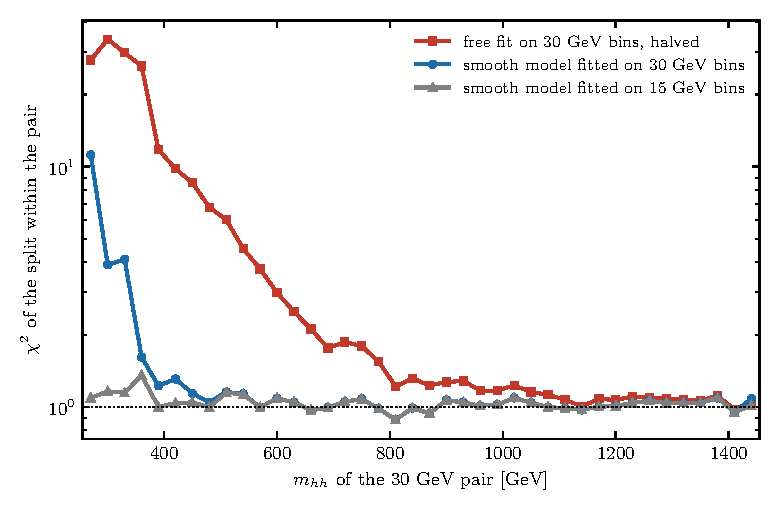
\includegraphics[width=0.62\textwidth]{fig_smooth_merged.pdf}
\caption{$\chi^2$ of the split of each 30-GeV pair into its two 15-GeV bins on the test spectra.
1 is perfect.}
\label{fig:merged}
\end{figure}

Above about 360~GeV the smooth model fitted on 30-GeV bins predicts the split as well as the
model fitted on 15-GeV bins ($\chi^2 \approx 1.0$--1.2), where the halved free fit gives up to
30 (\cref{fig:merged}). In the first three pairs (255--345~GeV) the split $\chi^2$ is 11, 3.9
and 4.1: the threshold rise has structure on scales below 30~GeV that 30-GeV data cannot fix.
Overall, the deviance of the 15-GeV predictions below 555~GeV is 2.34 for the smooth model
fitted on 30-GeV bins, 9.35 for the halved free fit and 1.57 for the smooth model fitted on
15-GeV bins.

% ===========================================================================
\section{The edges: 240--255 and 1455--1500 GeV}

The POWHEG source files contain the bins 240--255 and 1455--1500~GeV, which were not used.

\begin{table}[h]
\centering
\small
\begin{tabular}{lcc}
\toprule
 & 240--255 GeV & 1455--1500 GeV \\
 & \multicolumn{2}{c}{observed/predicted, summed over the 1,000 test spectra} \\
\midrule
$J = 40$, threshold factor & 0.92 & 1.44 \\
$J = 40$, no threshold factor & 0.65 & 1.42 \\
$J = 30$, threshold factor & 0.83 & 1.05 \\
$J = 60$, threshold factor & 0.96 & 1.07 \\
\bottomrule
\end{tabular}
\caption{Extrapolation to the unused edge bins.}
\label{tab:edge}
\end{table}

Below the fitted range, the threshold factor makes the difference: without it the model
over-predicts 240--255~GeV by 55\%, with it by 4--20\%. Above the fitted range the prediction
depends on $J$ (5--44\% low): there the splines are fixed by the prior alone, and the quoted
uncertainties are correspondingly large (pull s.d.\ 0.3--0.9). \textbf{The model should be used
within 250--1455~GeV only.}

% ===========================================================================
\section{The coefficient functions}

\begin{figure}[p]
\centering
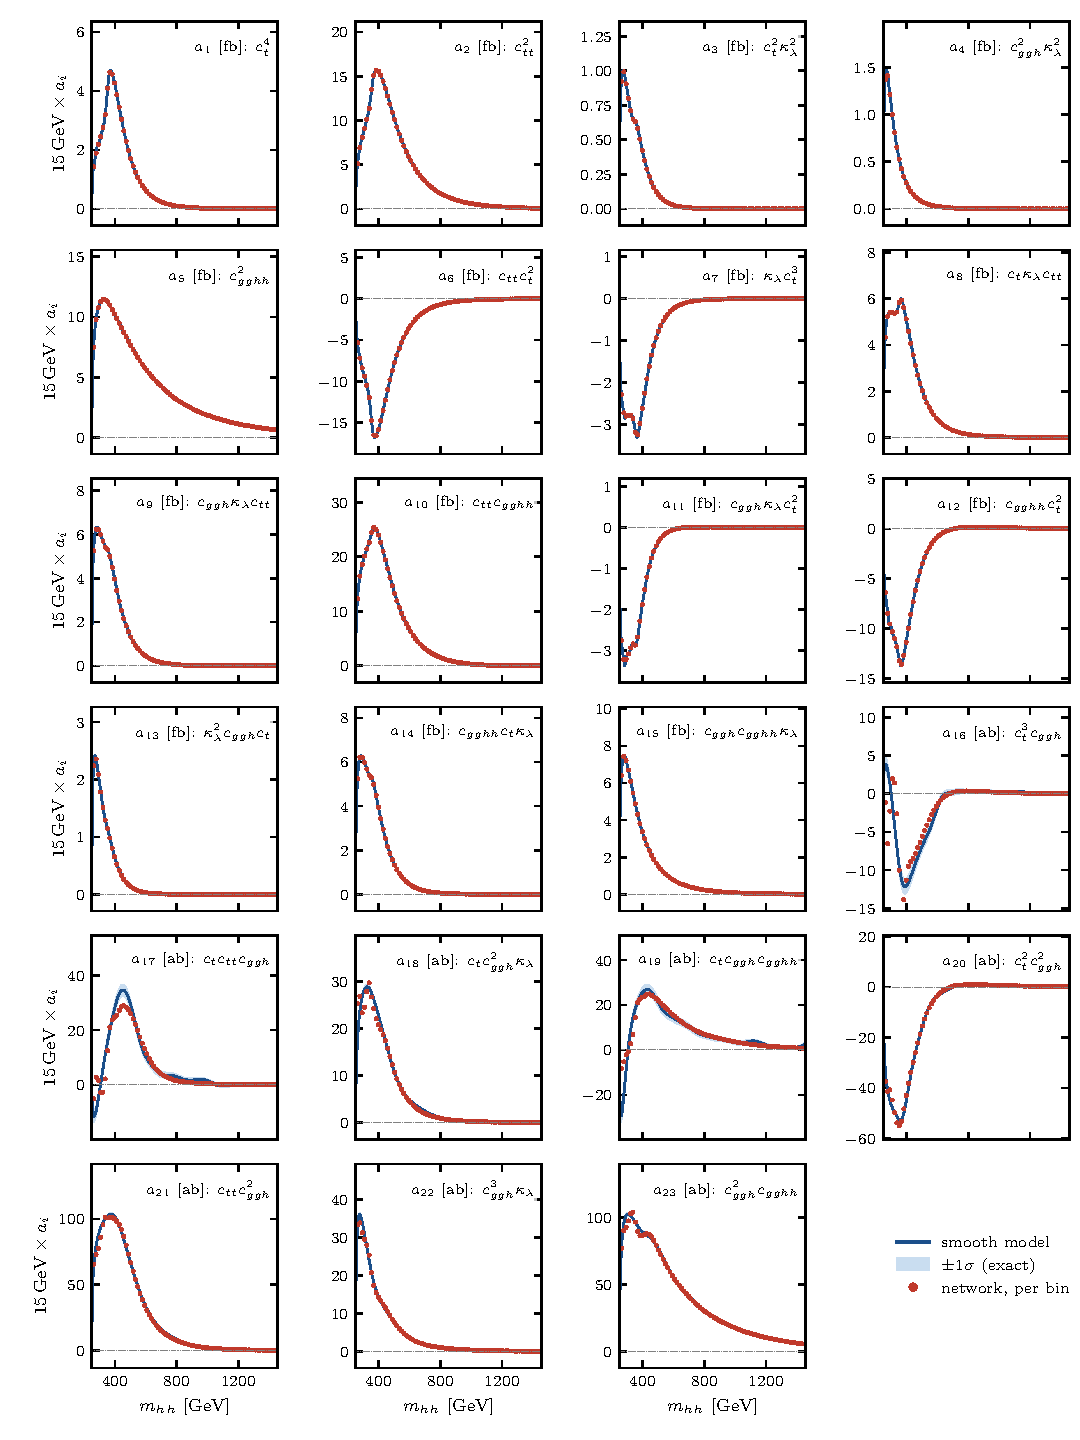
\includegraphics[width=\textwidth]{fig_smooth_coefficients.pdf}
\caption{The 23 coefficient functions, as $15\,\text{GeV}\times a_i(m_{hh})$ (the cross section
per 15~GeV), with their exact $\pm1\sigma$ bands, and the per-bin values of the network
ensemble (red points).}
\label{fig:coef}
\end{figure}

\Cref{fig:coef}: the smooth model and the network agree closely for $a_1$--$a_{15}$ and
$a_{21}$--$a_{23}$. The poorly determined $a_{16}$--$a_{20}$ are better determined than in the
network (median relative uncertainty 0.74, 0.37, 0.24, 0.21, 0.22 against 0.96, 1.34, 0.23,
0.21, 0.21), and differ from the network where both are uncertain. The roughness of the bin
values (rms second difference relative to the function's size) is 0.058, against 0.059 for the
network and 0.070 for the free fit. The data determine about 600 combinations of the 920
parameters; for $a_1$--$a_{15}$ 27--33 of the 38 curvature directions are determined (the
smoothness prior matters little), for $a_{16}$--$a_{23}$ only 12--23 of them.

% ===========================================================================
\section{Sensitivity}

\begin{itemize}
  \item \textbf{Number of splines}: $J$ = 30, 40, 60 give the same accuracy and calibration
    within 0.01 (\cref{tab:acc}). The evidence prefers $J = 40$ (by 47 and 250 units of
    $\ln Z$ over 30 and 60) in the first pass.
  \item \textbf{Threshold factor}: no effect within 255--1455~GeV; decisive below 255~GeV
    (\cref{tab:edge}). The evidence, computed only on 255--1455~GeV, is slightly higher without
    it; the edge test is the better guide.
  \item \textbf{Second pass} (the discrepancy in the weights): calibration unchanged (pull s.d.\
    1.003), but the raw agreement near threshold worsens (deviance 1.87 against 1.57), because the
    cancelling spectra, which are given less weight, are fitted less closely, and the test
    spectra share their peculiarity. Since the purpose of the model is to reproduce POWHEG, we
    recommend the first pass as the primary model, and the difference between the passes as a
    measure of how much the $a_i$ depend on the treatment of the cancelling spectra.
\end{itemize}

% ===========================================================================
\section{Next steps}

\begin{enumerate}
  \item Make the smooth model the primary model in the paper: rewrite the appendix around it,
    remake the figures (the 9-panel spectra with the continuous density, the coefficient
    functions of \cref{fig:coef}, all test spectra), update the executive summary.
  \item Note the weighting bias in the paper, and, for the cross-check, either refit the network
    fine-tune with Poisson weights or state the bias.
  \item The discrepancy correlated in $m_{hh}$ (a Gaussian process), needed for predictions summed
    over many bins.
  \item The questions to the generator side (\file{docs/modelerror/model_error_note.pdf}),
    now including the steep rise of $\varepsilon$ at high mass.
  \item Optionally, finer knots near threshold, which the merged-bin test suggests could help
    below 345~GeV.
\end{enumerate}

\paragraph{Code.} \file{dihiggs/smooth.py}; \file{code/smooth_toy.py}; \file{code/heft_smooth.ipynb}
(fit, validation, coefficient functions; writes \file{runs/SMOOTH_J40/}); the analysis scripts of
this note are in \file{docs/smooth/scripts/}.

\end{document}
